\documentclass{beamer}

\usepackage[utf8]{inputenc}
\usepackage{algorithm}
\usepackage{algpseudocode}
\usepackage{setspace}

\usetheme[%
    numbering=fraction,
    progressbar=foot,
]{metropolis}

\setbeamercolor{frametitle}{use=normal text}


\title{Twitter sentiment analysis with Hadoop}
\author{Emilio Cecchini}
\institute{
    Università degli Studi di Firenze \\
    \medskip
    \textit{emilio.cecchini@stud.unfi.it}
}
\date{\today}


\begin{document}


\maketitle


\begin{frame}{Overview}
\tableofcontents
\end{frame}


\section{Sentiment analysis}

\begin{frame}{Sentiment analysis}

\begin{itemize}
\item
Sentiment analysis involves classifying opinions in text into categories like \textit{positive} or \textit{negative} often with an implicit category of \textit{neutral}.
\item
In this project, for simplicity, we will ignore the \textit{neutral} category.
\item
All the entire part of building the classifier and getting results out of it is done with the LingPipe library, so we will ignore the internal details of the classifier.
\end{itemize}

\end{frame}


\begin{frame}{Training phase}
First of all there is a \textit{training} phase, where the model is trained to recognize a tweet as negative or positive. This phase is only implemented in a sequential version.
\end{frame}


\begin{frame}{Classification phase}
Once the model is built and trained, there is the \textit{classification} phase, where many unclassified tweets are passed as input to the model. This phase is implemented in two different versions: a sequential version and a distributed version in Hadoop with the MapReduce framework.
\end{frame}


\section{Training the model}


\begin{frame}{The training process}

\begin{itemize}
\item
The training process is done with a dataset containing tweets already classified.
\item
The model reads the tweet texts and their sentiment and try to learn how to perform the classification.
\item
The process of training the model must be computed in a sequential way because every tweet and its associated sentiment must be processed by the same unique model. A parallel version could be hypothetical possible but in that case reading and processing the tweet must be encapsulated in a critical section and therefore all the advantages of parallelization would be lost.
\end{itemize}

\end{frame}


\begin{frame}[fragile]{The training process}

Thanks to the LingPipe library, the algorithm of training the model is straightforward:

\begin{algorithm}[H]
\caption{Training the model}
\textbf{Input:} a list of tweets $T$ with text and sentiment. \\
\begin{algorithmic}
    \State $m$ = initializeModel()
    \For{each $t \in T$}
        \State handle($m$, $t$)
    \EndFor
    \State saveModel($m$)
\end{algorithmic}
\end{algorithm}

The function \verb"saveModel()" save the model in a file so that it can be loaded later by a classifier to perform a classification.

\end{frame}


\section{Sequential classification}


\begin{frame}{Sequential classification}

\begin{itemize}
\item
With the LingPipe library it is very easy to implement a sequential algorithm that classify tweets.
\item
The first thing to do is to load the trained model. This process may take a long time if the model has been trained with a very large dataset. Loading the model can not be parallelized, so it is suggested to keep the file as small as possible to prevent it to become the bottleneck of the program.
\item
After loading the model, the program iterates over the tweet texts and uses the classifier to predict their sentiment. During the iteration, the program keep tracks of the number of negative tweets as well as the number of positive tweets with two counters.
\end{itemize}

\end{frame}


\begin{frame}[fragile]{Sequential classification}

\begin{algorithm}[H]
\caption{Sequential classification}
\footnotesize
\textbf{Input:} a list of tweets $T$ with text only. \\
\textbf{Output:} two values $p, n \in \mathbb{N}$ that are the number of tweets classified as positives or negatives respectively. \\
\begin{algorithmic}

\State $m$ = loadModel()
\State $p$ = 0
\State $n$ = 0
\For{each tweet $t$}
    \State $s$ = classify($m$, $t$)
    \If{isPositiveSentiment($s$)}
        \State $p$ = $p$ + 1
    \Else
        \State $n$ = $n$ + 1
    \EndIf
\EndFor
\State \Return $p$, $n$

\end{algorithmic}
\end{algorithm}

\end{frame}


\section{Hadoop and the MapReduce framework}


\begin{frame}{Hadoop}
The classification process can be improved by implementing a distributed algorithm. This project uses Hadoop with its \textit{Hadoop Distributed File System} (HDFS) in order to better handle large amounts of data.
\end{frame}


\begin{frame}{MapReduce framework}

\begin{itemize}
\item
A MapReduce program is composed by a \textit{map} phase and by a \textit{reduce} phase.
\item
The map function processes each element of the input and returns a value associated with a key.
\item
The reduce function takes as input the keys returned by the map function and their associated values and then it combines them in a single value.
\end{itemize}

\end{frame}


\section{Distributed classification}


\begin{frame}{Distributed Cache}

\begin{itemize}
\item
In order to perform the classification of a tweet the model must first be loaded.
\item
This implementation exploits the \textit{Distributed Cache} tool to make the file where the model is stored accessible to all the map tasks.
\item
The Distributed Cache is a read-only data structure from which each application in the MapReduce framework can read files. Each map task loads its own model so there are not synchronization issues such as race conditions.
\end{itemize}

\end{frame}


\begin{frame}{Map phase}

Once the model is loaded from its file we can perform the map phase, which consists of mapping each tweet text to its classified sentiment.

\begin{algorithm}[H]
\caption{Map function}
\textbf{Input:} a trained model $m$, a tweet text $t$ \\
\textbf{Output:} a key $k$ and a value $v = 1$ \\
\begin{algorithmic}
    \State s = classify($m$, $t$)
    \If{isPositiveSentiment($s$)}
        \State $k$ = \textit{positives}
    \Else
        \State $k$ = \textit{negatives}
    \EndIf
    \State \Return $k$, 1

\end{algorithmic}
\end{algorithm}

\end{frame}


\begin{frame}{Reduce phase}

The reduce function takes as input the key and a list of as many ones as many tweets have been classified in that category.

\begin{algorithm}[H]
\caption{Reduce function}
\textbf{Input:} a key $k$ and a list $V$ of values $v = 1$ \\
\textbf{Output:} a key $k$ and a value $c$ \\
\begin{algorithmic}
    \State $c$ = 0
    \For{each element in $v \in V$}
        \State c = c + 1
    \EndFor
    \State \Return $k$, $c$
\end{algorithmic}
\end{algorithm}

The only thing that the reduce function has to do is to count the number of elements that are in the list associated with the input key.

\end{frame}


\begin{frame}{Partitioner}

\begin{itemize}
\item
Since the keys that the mapper passes to the reducer are always two (\textit{positive} or \textit{negatives}), the number of reducers can be specified at compilation time to two.
\item
To optimize the operations of dispatching the mapper output, a \textit{partition} function is implemented.
\item
The purpose of this function is to assign the output key of a map function to a specific reducer.
\end{itemize}

\end{frame}


\begin{frame}{Partitioner}
Since we have set the number of reducers to two, the output of this function is 1 or 0 dependending if the key is \textit{positives} or \textit{negatives}.

\begin{algorithm}[H]
\caption{Partion function}
\textbf{Input:} a key $k$ \\
\textbf{Output:} a value $v$ \\
\begin{algorithmic}
    \If{$k$ == "positives"}
        \State \Return 1
    \ElsIf{$k$ == "negatives"}
        \State \Return 0
    \Else
        \State \Return -1 \Comment{Error}
    \EndIf
\end{algorithmic}
\end{algorithm}

\end{frame}

\section{Speedup}

\begin{frame}{Speedup}
The \textit{speedup} is the ratio between the execution time of the sequential version and the execution time of the parallel version with the same input.

\begin{align*}
S = \dfrac{t_S}{t_P}
\end{align*}

Ideally, the speedup should be the number of processor used to perform the parallel version. For a distributed algorithm, it should be the number of nodes in the cluster.
\end{frame}


\begin{frame}{Experiments setup}

\begin{itemize}
\item
The inputs for these experiments are some text files containing the tweet texts.
\item
The size of a single text file is about the size of a HDFS block, that is 128 MB by default. This make it easier to control the number of splits into which the input will be divided.
\item
In order to see the trend of the speedup, we tested the distributed algorithm in a cluster with a different number of nodes, more precisely from two to five nodes.
\item
Each node has an Intel Haswell CPU with four cores and 8 GB of RAM.
\end{itemize}

\end{frame}


\begin{frame}{Input size = 1}
\begin{figure}[H]
\centering
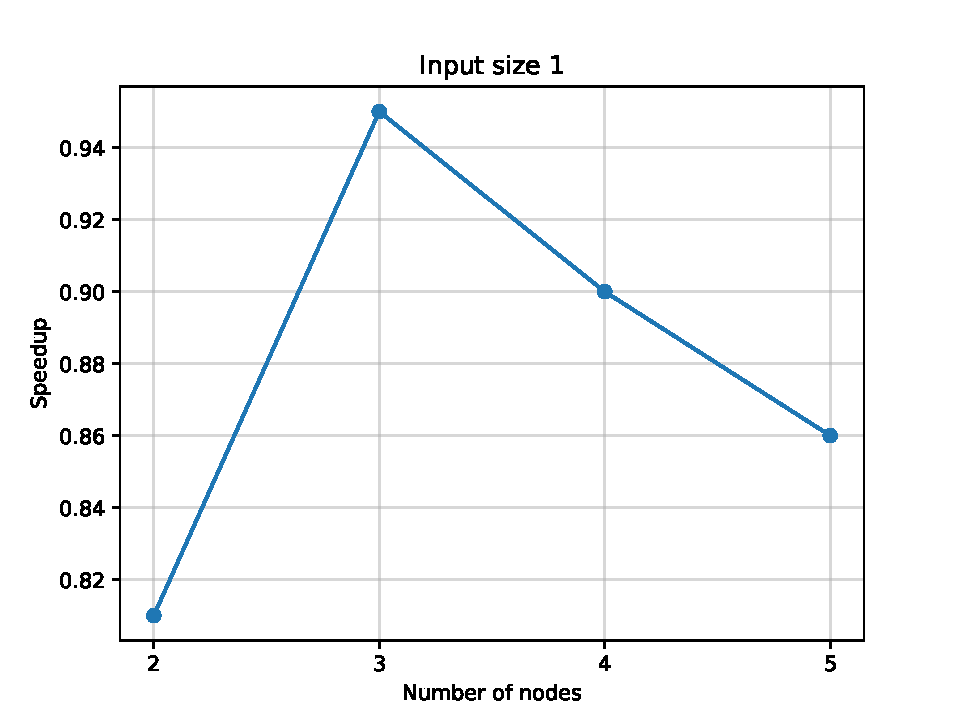
\includegraphics[width=3.2in]{../Paper/fig/speedup1}
\end{figure}
\end{frame}


\begin{frame}{Input size = 5}
\begin{figure}[H]
\centering
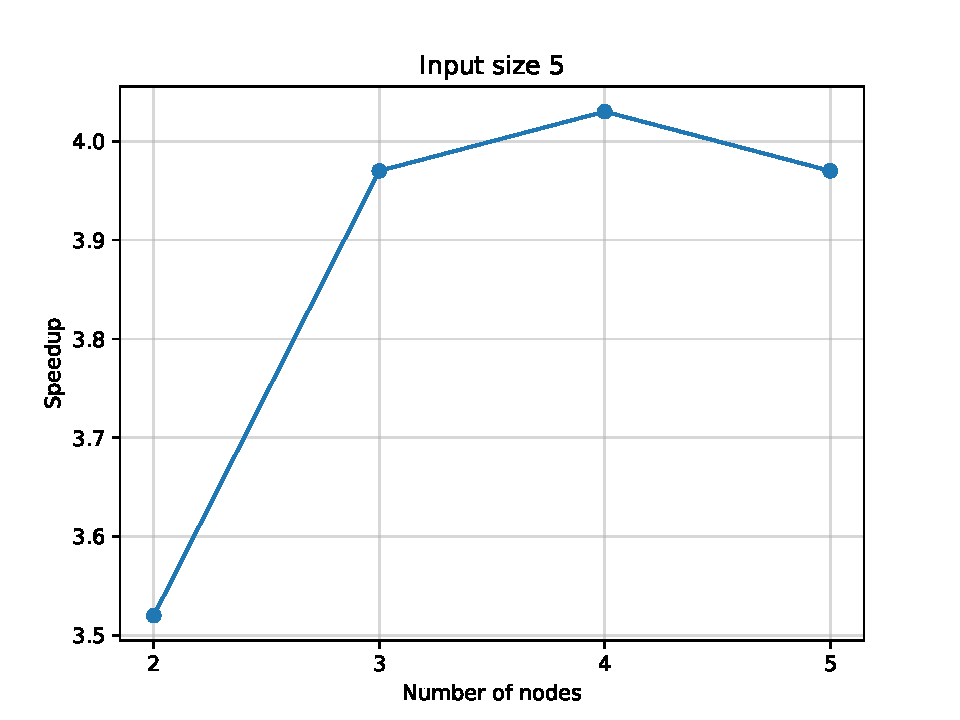
\includegraphics[width=3.2in]{../Paper/fig/speedup5}
\end{figure}
\end{frame}


\begin{frame}{Input size = 10}
\begin{figure}[H]
\centering
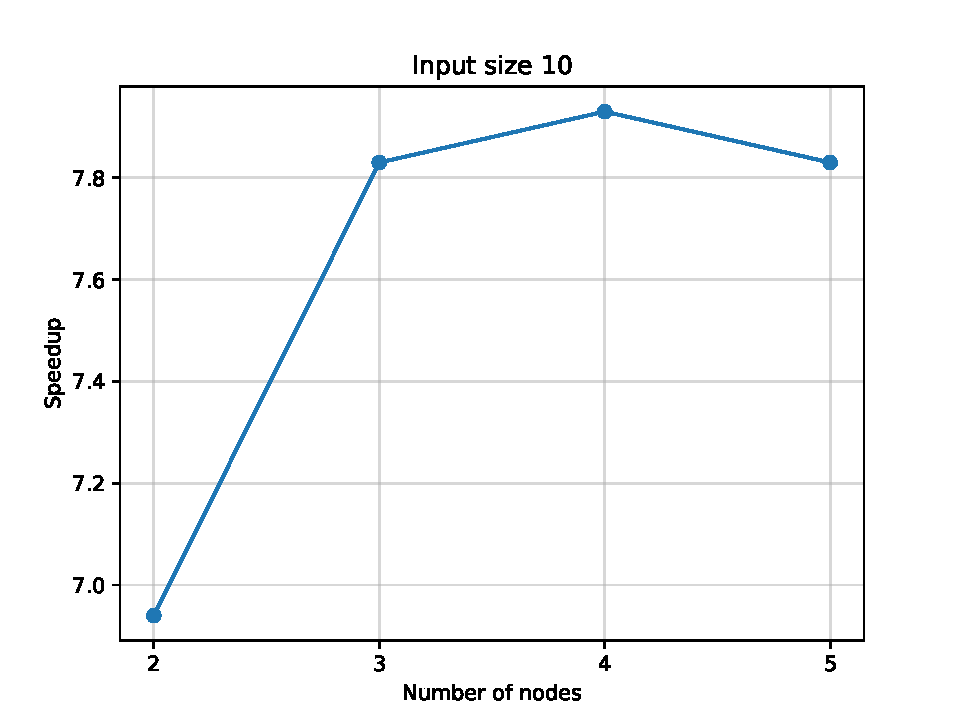
\includegraphics[width=3.2in]{../Paper/fig/speedup10}
\end{figure}
\end{frame}


\begin{frame}{Input size = 20}
\begin{figure}[H]
\centering
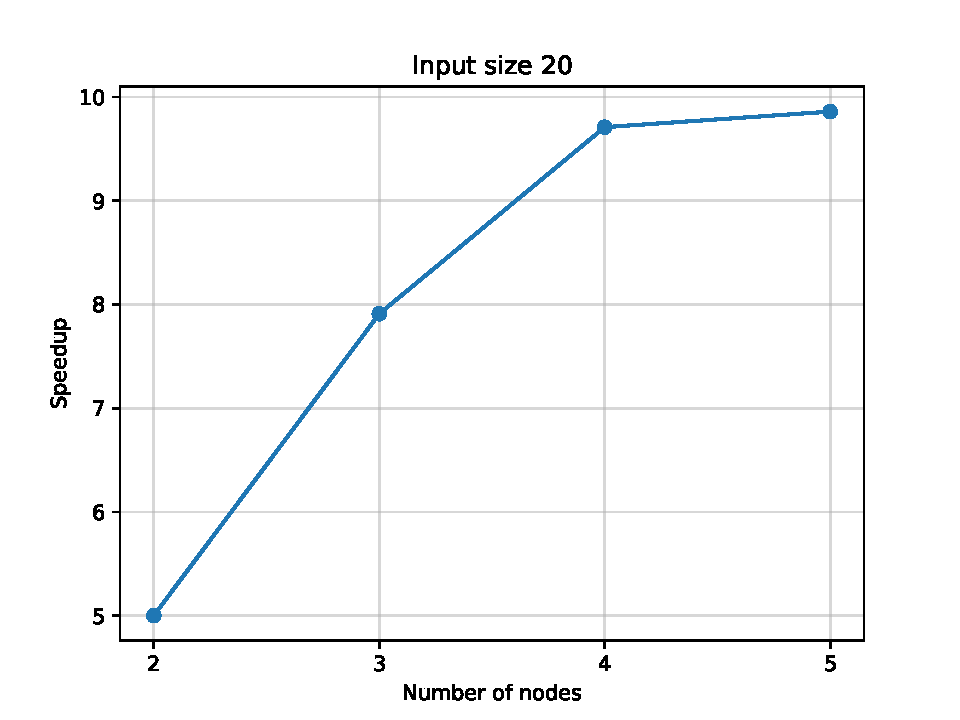
\includegraphics[width=3.2in]{../Paper/fig/speedup20}
\end{figure}
\end{frame}

\begin{frame}{Conclusion}

\begin{itemize}
\item
From these simple experiments we can confirm that Hadoop is designed to work with big data, because if the input size is too small we have a lot of overhead due to tasks management.
\item
Apart from the first case, where we passed only a single file to the classifier, the speedups are always super-linear, that means that the speedup is alway greater then the number of nodes in the clusters.
\end{itemize}

\end{frame}

\end{document}
